\documentclass[11pt]{article}

\usepackage[T1]{fontenc}
\usepackage[utf8]{inputenc}
\usepackage{lmodern}
\usepackage[margin=1in]{geometry}
\usepackage{amsmath,amssymb,amsthm}
\usepackage{graphicx}
\usepackage{float}
\usepackage{booktabs}
\usepackage{enumitem}
\usepackage{microtype}
\usepackage{xcolor}
\usepackage{tikz}
\usetikzlibrary{arrows.meta,positioning}
\usepackage[colorlinks=true,linkcolor=blue!50!black,urlcolor=blue!50!black,citecolor=blue!50!black]{hyperref}

\newtheorem*{fact}{Fact}

\newcommand{\G}{\mathbb{G}}
\newcommand{\Z}{\mathbb{Z}}
\newcommand{\norm}{\operatorname{norm}}
\newcommand{\site}{\texttt{private-set-intersection.xyz}}

\title{Counting Shared Applicants Without Sharing Names\\[4pt]
  \large How \site{} works}
\author{Jim Fowler}
\date{\today}

\begin{document}
\maketitle

\begin{abstract}
  Summer mathematics programs want to know how much their applicant pools overlap. How many
  distinct students apply across all of our programs? Which pairs of programs share many
  applicants? To how many programs does a typical student apply? But no program can hand its list of
  applicants to another program, or to a third party. This note describes a protocol, and a website
  that implements it, that answers these questions while every list of names stays on its owner's
  computer. The method is the classical Diffie--Hellman \emph{private set intersection}: each program
  scrambles names with a secret key, every program applies its key to every list, and because
  the scrambling commutes, equal names end up as equal scrambled values. Then we can count
  collisions, but no one can learn which names collided.
\end{abstract}

\tableofcontents

%======================================================================
\section{The question}
%======================================================================

Each participating program $X$ has a list $A_X$ of applicants. We would like to learn things like:
\begin{itemize}[nosep]
  \item the size of the union $\bigl|\bigcup_X A_X\bigr|$, i.e., the number of distinct applicants;
  \item the pairwise overlaps $|A_X \cap A_Y|$;
  \item the distribution of $m(s) = \#\{X : s \in A_X\}$, the number of programs to which student $s$ applies;
  \item more generally, for every set $S$ of programs, how many students applied to exactly the programs in $S$.
\end{itemize}
All of these quantities come from inclusion--exclusion counts. If a trusted party held every list,
the computation would be trivial. The difficulty is that \emph{nobody should hold every list}.
Applicant names are personal information about minors, many programs promise in their privacy
policies not to share applicant information, and it would be an uncomfortable precedent even
where it is permitted.

\subsection*{Why not just hash the names?}

A natural first idea is for every program to apply a public hash function $h$ (say SHA-256) to each
name and share the hashes. This does not protect anything. There are not that many names: anyone
holding the hashed lists can hash every plausible ``First Last'' pair (or simply the names of
their own applicants) and look the results up. Hashing with a public function is, for this
purpose, the same as sharing the names.

What we need is a scrambling function that
\begin{enumerate}[nosep]
  \item no single party can evaluate on its own (so no dictionary attack is possible), and yet
  \item produces the same output for the same name, no matter which program's list it came from.
\end{enumerate}
\emph{Commutative} encryption provides exactly this.

%======================================================================
\section{The protocol}
%======================================================================

\subsection{Ingredients}

Let $\G$ be a cyclic group of prime order $\ell$ in which the Diffie--Hellman problem is hard. We use
\textbf{ristretto255}~\cite{rfc9496}, a prime-order group built from Curve25519, with order
\[
  \ell = 2^{252} + 27742317777372353535851937790883648493 .
\]
Elements are encoded as 32 bytes.
We also need a hash function $H$ from strings to $\G$; we use the standard
\texttt{hash\_to\_ristretto255} construction of RFC~9380~\cite{rfc9380} (SHA-512 based), with a
domain-separation tag specific to this project. In the analysis, $H$ is modeled as a random
oracle: $H(x)$ behaves like a uniformly random group element.

Each program $i$ chooses a secret key $k_i \in \{1, \dots, \ell-1\}$ uniformly at random. To
\emph{encrypt} a group element $P$ with key $k$ means to compute the scalar multiple $kP$. (In
multiplicative notation, this is $P \mapsto P^{k}$, exactly as in Diffie--Hellman key exchange.)

\begin{fact}[Commutativity]
  For all keys $a,b$ and all $P \in \G$, we have $a(bP) = (ab)P = b(aP)$.
  So applying keys $k_1, \dots, k_n$ in \emph{any} order sends $P$ to $(k_1 k_2 \cdots k_n) P$.
\end{fact}

\noindent Since $\ell$ is prime and $k \not\equiv 0$, the map $P \mapsto kP$ is a bijection of $\G$, so
distinct names remain distinct at every stage.

\subsection{Steps}

Write $K = k_1 k_2 \cdots k_n \bmod \ell$. Each program $i$ with (normalized, deduplicated) list
$A_i$ does the following.

\begin{enumerate}
  \item \textbf{Upload.} Compute $\{\, k_i\, H(x) : x \in A_i \,\}$, shuffle it into a random order, and upload it.
  \item \textbf{Process.} Repeatedly: download any list that has not yet been touched by key $k_i$,
        multiply every element by $k_i$, shuffle, and upload the result in its place.
\end{enumerate}

\noindent When every program has touched every list, program $i$'s list has become
\[
  L_i = \{\, K\, H(x) : x \in A_i \,\}
\]
(shuffled), \emph{regardless of the order in which programs processed it}. Two programs' final lists
contain the same element exactly when they contain the same normalized name (up to the negligible
chance of a hash collision). The analysis is just counting:
\[
  |A_X \cap A_Y| = |L_X \cap L_Y|, \qquad
  \Bigl|\bigcup_X A_X\Bigr| = \Bigl|\bigcup_X L_X\Bigr|, \qquad \text{and so on.}
\]

\begin{figure}[ht]
\centering
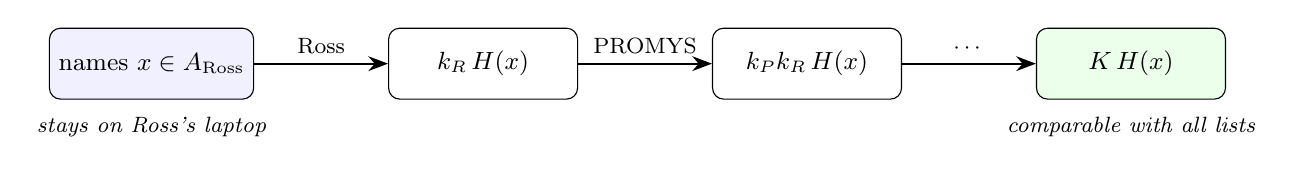
\begin{tikzpicture}[
    box/.style={draw, rounded corners, minimum height=9mm, minimum width=24mm, align=center, font=\small},
    arr/.style={-{Stealth[length=2.5mm]}, thick},
    lab/.style={font=\footnotesize, midway, above}]
  \node[box, fill=blue!6] (a) {names $x\in A_{\mathrm{Ross}}$};
  \node[box, right=17mm of a] (b) {$k_R\,H(x)$};
  \node[box, right=17mm of b] (c) {$k_P k_R\,H(x)$};
  \node[box, right=17mm of c, fill=green!8] (d) {$K\,H(x)$};
  \draw[arr] (a) -- node[lab]{Ross} (b);
  \draw[arr] (b) -- node[lab]{PROMYS} (c);
  \draw[arr] (c) -- node[lab]{$\cdots$} (d);
  \node[below=1mm of a, font=\footnotesize\itshape] {stays on Ross's laptop};
  \node[below=1mm of d, font=\footnotesize\itshape] {comparable with all lists};
\end{tikzpicture}
\caption{One program's list moving through the protocol. Every arrow is a scalar multiplication
followed by a shuffle. Other lists pass through the same keys in different orders and reach the
same final form.}
\end{figure}

\subsection{Why shuffle?}

If lists kept their order, a program that saw its own list both before and after another program's
key was applied could match positions and learn which of its applicants are which encrypted values.
Shuffling at every step breaks that link. In addition, the server only gives a program lists it has
\emph{not yet} processed, and never gives a program its own list back after uploading it.

\subsection{Why deduplicate?}

Every list is deduplicated (after normalization) before upload. If a list could contain the same
encrypted value twice, a program with two applicants of the same name would recognize the pair in
the final data.

%======================================================================
\section{What each party learns}
%======================================================================

The security of the scheme rests on the Decisional Diffie--Hellman assumption in $\G$: given
$P$, $aP$, $Q$ and $R$, it is infeasible to decide whether $R = aQ$. Under this assumption, and
with $H$ modeled as a random oracle, a list encrypted under keys one does not know looks like
random group elements.

\begin{center}
\begin{tabular}{@{}p{0.2\linewidth}p{0.74\linewidth}@{}}
  \toprule
  \textbf{Party} & \textbf{Learns} \\
  \midrule
  Each program & Its own list (of course); the \emph{sizes} of other programs' lists; nothing about
                 the contents of other lists. \\
  The server   & Encrypted lists at every stage and each list's size and within-list duplicate
                 counts. It never sees a name or a key: keys are generated in the browser, and only
                 a public fingerprint $k_i G$ is stored, to catch someone loading the wrong key file. \\
  Organizers   & The final counts: union size, pairwise overlaps, and how many encrypted names fall
                 in each combination of programs. They can tell that \emph{some} student applied to
                 exactly Ross and PROMYS, but not who. \\
  \bottomrule
\end{tabular}
\end{center}

\subsection*{Limitations}

\begin{itemize}
  \item \textbf{Honest-but-curious.} The protocol assumes every program actually applies its key.
        Nothing \emph{proves} that a program multiplied by $k_i$ (the server checks only that it
        returned the right number of distinct, valid group elements). A single program that cheats
        is most likely to corrupt the results. Using cheating to learn about another program's
        applicants would take more, such as the fake second participant described next.
  \item \textbf{Fake participants.} Someone who registers a second, fake ``program'' controls two
        keys and could probe whether particular names appear on other lists. Registration
        therefore requires a join code distributed by the organizers, and the organizers can close
        registration once every real program has joined.
  \item \textbf{Small cells.} When many programs participate, some combinations will contain only
        one or two students. These counts are visible only to the organizers, who should avoid
        publishing small cells.
  \item \textbf{Names are an imperfect identifier.} See the next two sections.
\end{itemize}

%======================================================================
\section{Normalizing names}
%======================================================================

The protocol compares strings exactly, so the same student must produce the same string at every
program. Different programs store names differently (one field or two, last-name-first, middle
initials, nicknames in parentheses), so before hashing, every name is normalized in the browser:

\begin{enumerate}[nosep]
  \item remove anything in parentheses or brackets, and quoted nicknames;
  \item strip accents ({\'e}$\to$e, {\~n}$\to$n);
  \item treat commas, tabs, and semicolons as spaces, and split into words;
  \item uppercase each word and delete punctuation inside it (so hyphens and apostrophes disappear);
  \item drop trailing generational suffixes (Jr, Sr, II, III, \dots);
  \item keep only the \emph{first} and \emph{last} remaining words;
  \item sort those two words alphabetically and join them.
\end{enumerate}

\noindent Sorting means we never need to know which word is the given name and which is the
family name, so ``Lee, Justin'' and ``Justin Lee'' agree.

\begin{center}
\begin{tabular}{@{}ll@{}}
  \toprule
  \textbf{Pasted} & \textbf{Normalized key} \\
  \midrule
  Jim Jordan                 & \texttt{JIM|JORDAN} \\
  Joe Jameson                & \texttt{JAMESON|JOE} \\
  Lee, Justin                & \texttt{JUSTIN|LEE} \\
  Justin Lee (1 of 2)        & \texttt{JUSTIN|LEE} \\
  Anne-Marie Dubois          & \texttt{ANNEMARIE|DUBOIS} \\
  Jos\'e N\'u\~nez           & \texttt{JOSE|NUNEZ} \\
  Matthew A.\ Husen Jr.      & \texttt{HUSEN|MATTHEW} \\
  \bottomrule
\end{tabular}
\end{center}

This deliberately introduces a few false matches. Two different students named Justin Lee become
one key, and so do ``Jim Jordan'' and ``Jordan Jim''. It also misses some true matches (``Matt
Smith'' versus ``Matthew Smith''). We ask programs to paste legal names, which removes most of the
second problem, and we \emph{measure} the first problem, as described next.

%======================================================================
\section{From distinct names to distinct people}
%======================================================================

Each program's own list is already a list of distinct \emph{people}. So when the browser normalizes
a list, every repeated key is a genuine name collision among distinct people. The browser
records the \emph{multiplicity spectrum}: for each $m \ge 1$, the number of keys that occur exactly
$m$ times in that list. Only these counts are uploaded.

Let $p_j$ be the fraction of applicants whose normalized name is $j$, and let
\[
  C_2 = \sum_j p_j^2,
\]
the probability that two randomly chosen applicants share a normalized name. From a list of $n$
people whose spectrum has $s_m$ keys of multiplicity $m$, the number of colliding pairs is
$\sum_m s_m\binom{m}{2}$ out of $\binom{n}{2}$ pairs. Pooling over programs gives the estimate
\[
  \widehat{C}_2 = \frac{\sum_{\text{programs}} \sum_m s_m \binom{m}{2}}{\sum_{\text{programs}} \binom{n}{2}}.
\]

Now suppose there are $N$ distinct people in total, and $U$ distinct normalized names in the
union. Name $j$ is absent from the union only if none of the $N$ people has it, so
\[
  \mathbb{E}[U] = \sum_j \bigl(1 - (1-p_j)^N\bigr)
  \approx \sum_j \Bigl(N p_j - \tbinom{N}{2} p_j^2\Bigr)
  = N - \tbinom{N}{2} C_2 ,
\]
using $\sum_j p_j = 1$. We therefore estimate the number of people by solving
\[
  N = U + \tbinom{N}{2}\,\widehat{C}_2
\]
by fixed-point iteration. In practice $C_2$ is on the order of $10^{-5}$ or smaller, so the
correction is small. That small size is itself useful to know: it tells us that ``matching by
name'' is accurate enough for the questions we are asking.

The same reasoning, applied with higher moments $C_r = \sum_j p_j^r$, could refine the estimate
and produce corrections for the pairwise counts. We have not needed this.

%======================================================================
\section{Using the website}
%======================================================================

All of the cryptography runs in the participant's browser, in a background thread (Web Worker).
The browser code is not minified, so anyone can read it with ``view source''. The server
(Node.js, Express, SQLite) stores only encrypted lists, counts, and a public key fingerprint per
program.

\subsection{Before the session}

Each program should prepare a plain-text list of applicant \textbf{legal names}, one per line,
first and last name in either order. Programs should leave duplicate names in, because the page
counts them, and need not clean up markers like ``(1 of 2)''. Optionally, programs can prepare two
lists, one of completed applications and one of all applicants. These are analyzed separately.

\subsection{Step 0: register}

One person per program registers with the program's name, a password, and the join code from the
organizers (Figure~\ref{fig:register}).

\begin{figure}[H]
  \centering
  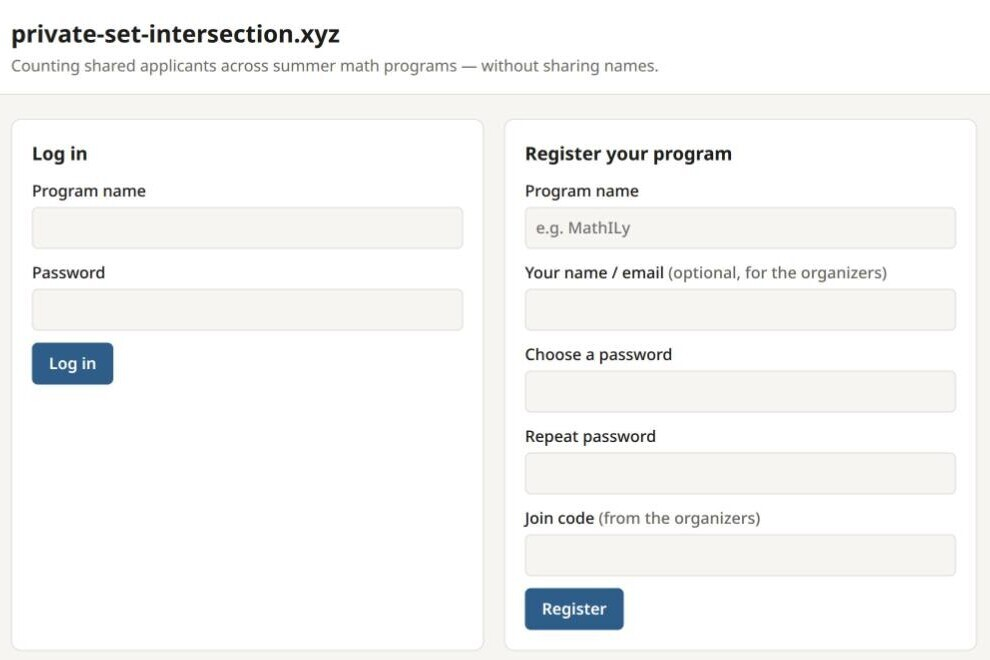
\includegraphics[width=0.8\linewidth]{figures/register.jpg}
  \caption{Logging in or registering a program.}
  \label{fig:register}
\end{figure}

\subsection{Step 1: generate a key}

The page generates the program's secret key, keeps it in the browser, and downloads a backup
copy (\texttt{psi-key-\emph{program}.json}). Keep this file until the exercise is over. If you
switch computers or browsers, load the backup and the page will verify that it matches. Do not send
the key to anyone, including the organizers.

\subsection{Step 2: paste and upload}

Paste the list. The page immediately shows how many distinct keys the list contains, how each name
is normalized, and which rows look suspicious, such as email addresses, digits, or single words
(Figure~\ref{fig:paste}). Fix anything that is wrong, then click \emph{Encrypt and upload}. The
names never leave the computer; only the encrypted points are uploaded.

\begin{figure}[H]
  \centering
  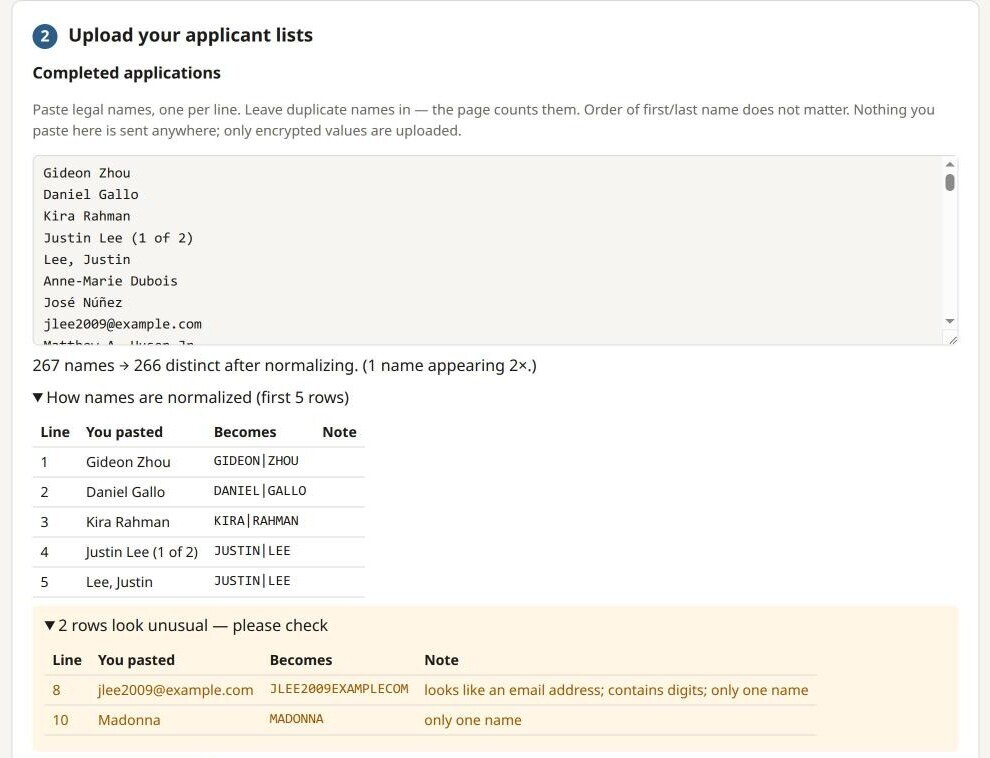
\includegraphics[width=0.8\linewidth]{figures/paste.jpg}
  \caption{Pasting a list. The two flagged rows are an email address and a single name, both
  probably mistakes.}
  \label{fig:paste}
\end{figure}

\subsection{Step 3: process everyone else's lists}

Click \emph{Start processing} and leave the tab open. The page repeatedly asks the server for a
list that still needs this program's key, applies the key, and uploads the result. There are no
fixed rounds: lists flow to whichever programs are ready. If two programs grab the same list at the
same moment, the server accepts only one result, and the other program simply moves on and retries
later. The progress board (Figure~\ref{fig:progress}) shows which program has processed which list,
so it is easy to see who is still working.

\begin{figure}[H]
  \centering
  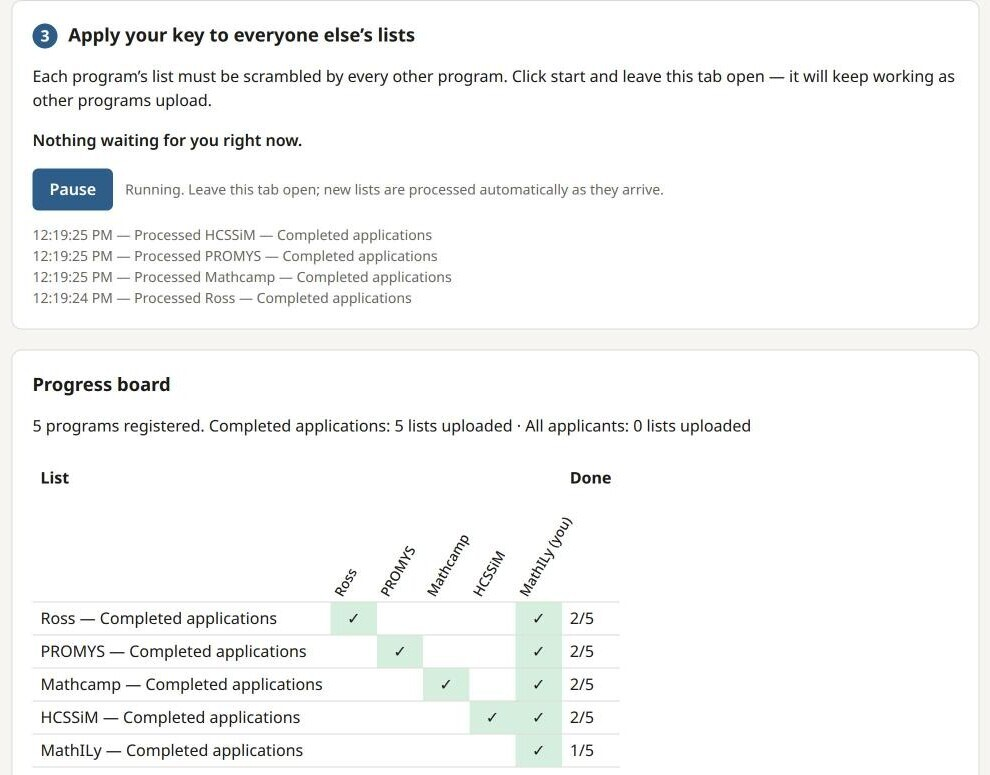
\includegraphics[width=0.8\linewidth]{figures/progress.jpg}
  \caption{Partway through: MathILy has applied its key to every list, but the other programs have
  not yet processed MathILy's list or one another's.}
  \label{fig:progress}
\end{figure}

\subsection{Results}

When every list has been processed by every program, the organizer page shows the results
(Figures~\ref{fig:results} and~\ref{fig:histogram}). These include:
\begin{itemize}[nosep]
  \item the union size and the estimated number of distinct people;
  \item for each program, how many applicants appear on no other list;
  \item the pairwise overlap matrix;
  \item the distribution of the number of programs per applicant;
  \item counts for every exact combination of programs.
\end{itemize}
The organizers can also download a de-identified CSV with one row per encrypted name and one 0/1
column per program, for further analysis.

\begin{figure}[H]
  \centering
  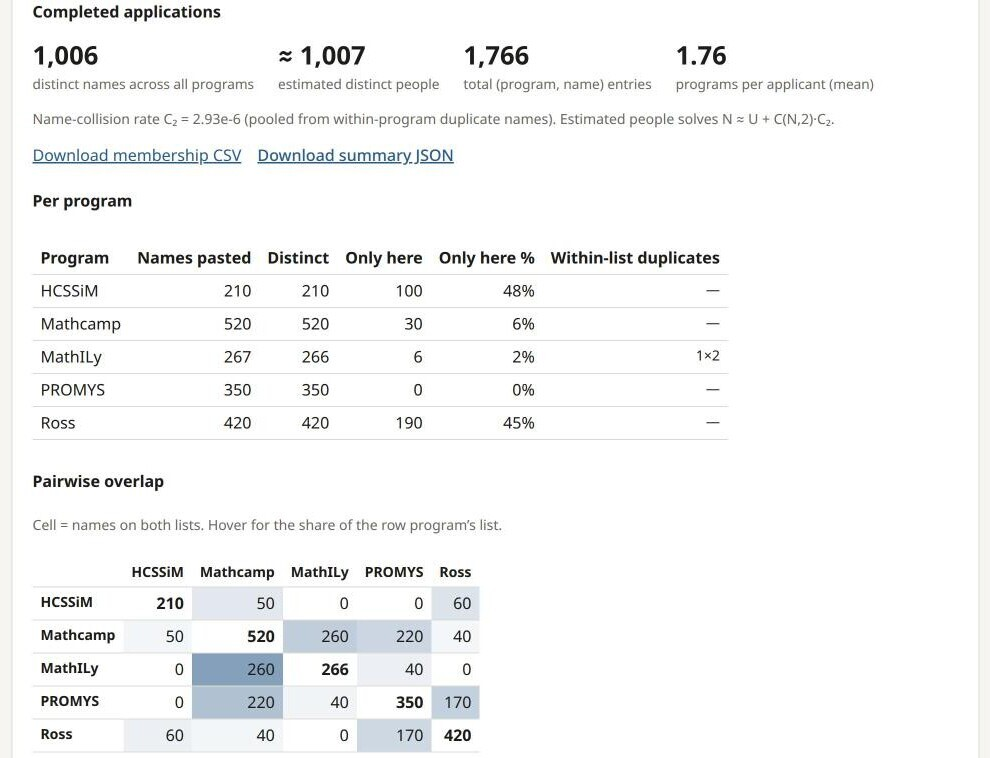
\includegraphics[width=0.8\linewidth]{figures/results.jpg}
  \caption{Organizer view of the results, using synthetic data for five programs.}
  \label{fig:results}
\end{figure}

\begin{figure}[H]
  \centering
  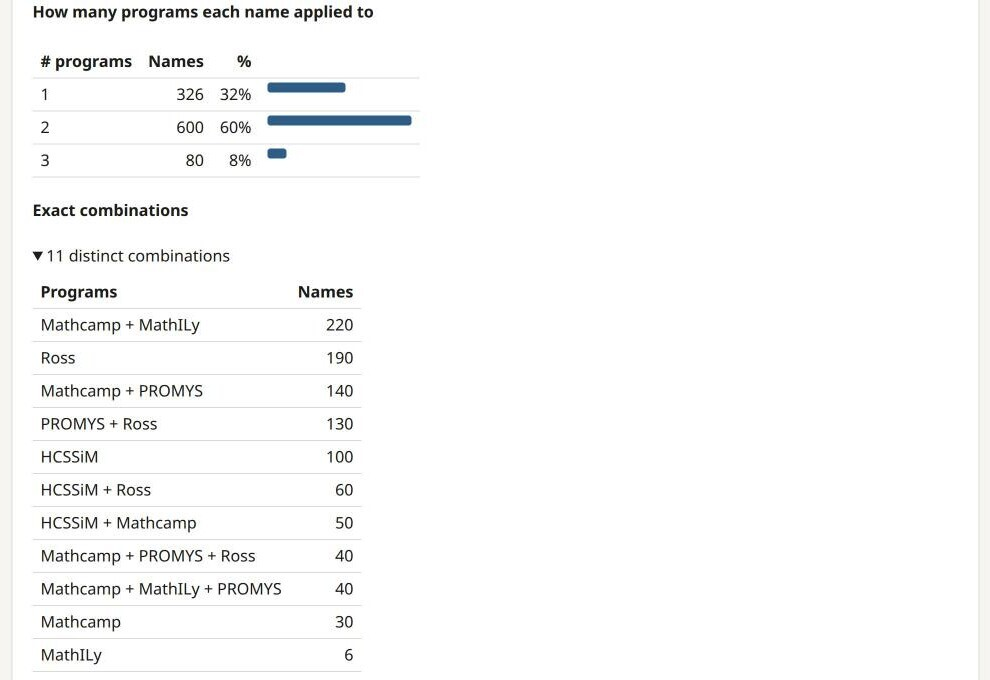
\includegraphics[width=0.8\linewidth]{figures/histogram.jpg}
  \caption{How many programs each (encrypted) name applied to, and the exact combinations.}
  \label{fig:histogram}
\end{figure}

%======================================================================
\section{Provenance}
%======================================================================

We did not invent this cryptography. Commutative-encryption set intersection goes back to
Meadows~\cite{meadows} and to Huberman, Franklin, and Hogg~\cite{hfh}, and it is a standard
example of private set intersection~\cite{psi-survey}. The group (ristretto255) and the hash-to-group
construction are IETF standards~\cite{rfc9496,rfc9380}, and the implementation uses the audited
\texttt{@noble/curves} library~\cite{noble}. The source code for the website is at
\url{https://github.com/kisonecat/private-set-intersection.xyz}.

\begin{thebibliography}{9}
\bibitem{meadows}
  C.~Meadows, ``A more efficient cryptographic matchmaking protocol for use in the absence of a
  continuously available third party,'' \emph{IEEE Symposium on Security and Privacy}, 1986.
\bibitem{hfh}
  B.~A.~Huberman, M.~Franklin, and T.~Hogg, ``Enhancing privacy and trust in electronic
  communities,'' \emph{ACM Conference on Electronic Commerce}, 1999.
\bibitem{psi-survey}
  B.~Pinkas, T.~Schneider, and M.~Zohner, ``Scalable private set intersection based on OT
  extension,'' \emph{ACM Transactions on Privacy and Security} 21(2), 2018. See also
  \url{https://en.wikipedia.org/wiki/Private_set_intersection}.
\bibitem{rfc9496}
  H.~de~Valence, J.~Grigg, M.~Hamburg, I.~Lovecruft, G.~Tankersley, and F.~Valsorda,
  ``The ristretto255 and decaf448 Groups,'' RFC~9496, 2023.
\bibitem{rfc9380}
  A.~Faz-Hern\'andez, S.~Scott, N.~Sullivan, R.~S.~Wahby, and C.~A.~Wood,
  ``Hashing to Elliptic Curves,'' RFC~9380, 2023.
\bibitem{noble}
  P.~Miller, \texttt{noble-curves}, \url{https://github.com/paulmillr/noble-curves}.
\end{thebibliography}

\end{document}
